% DO NOT COMPILE THIS FILE DIRECTLY!
% This is included by the other .tex files.


\begin{frame}
    
\includegraphics[scale=0.3]{images/logo-circl-Forensics.png}
    \begin{itemize}
        \item[]
        \item[]
        \item[] 5. Disk Analysis
    \end{itemize}
\end{frame}


\begin{frame}
  \frametitle{5.1 CHS - Cylinder Head Sector}
    \begin{itemize}
        \item[] Track, Head, Cylinder, Sector, Block, Cluster
    \end{itemize}
    \begin{figure}
        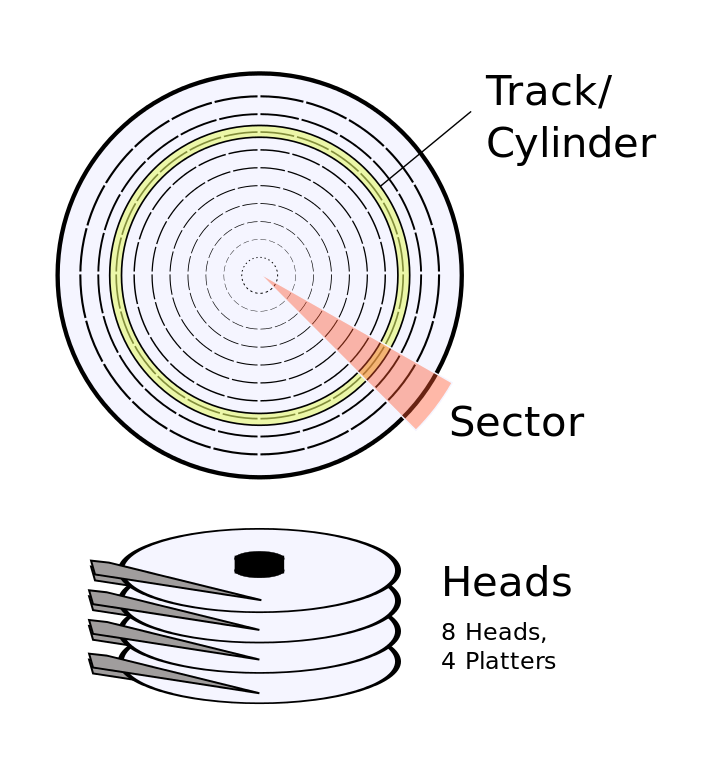
\includegraphics[scale=0.2]{images/chs.png}
        \captionsetup{labelformat=empty,labelsep=none}
        \transparent{0.4}%
        \caption[]{\tiny Image (c) wikipedia.org - Image used solely for illustration purposes}
    \end{figure}
\end{frame}


\begin{frame}[fragile]
  \frametitle{5.2 LBA - Logical Block Addressing}
  \begin{lstlisting}[basicstyle=\tiny\ttfamily]
Logical volume addresses
----------------------------------------------------------------------------
|  0 |  1 |  2 |  3 |  4 |  5 |  6 |  7 |  8 |  9 | 10 | 11 | 12 | 13 | 14 |
----------------------------------------------------------------------------
          |                   |                   |                   |
          |                   |                   |                   |
          -------------------------------------------------------------
   ^      |         0         |         1         |         3         |   ^
   |      -------------------------------------------------------------   |
   |      Logical file system addresses - Clusters                        |
  MBR                                                               Volume slack
          *-------------------*
               2.048 Bytes
          *-----------------------------------------------------------*
                                   6.144 Bytes
  \end{lstlisting}
\end{frame}


\begin{frame}[fragile]
  \frametitle{5.3 Low-Level: Sector Structur}
    \begin{figure}
        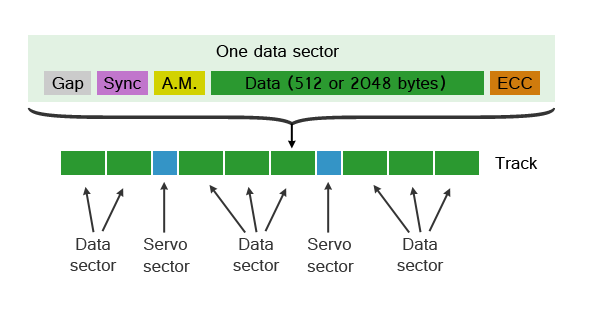
\includegraphics[scale=0.5]{images/sector.png}
        \captionsetup{labelformat=empty,labelsep=none}
        \transparent{0.4}%
        \caption[]{\tiny Image (c) forensicfocus.com - Image used solely for illustration purposes}
    \end{figure}
\end{frame}


\begin{frame}[fragile]
  \frametitle{5.3 Low-Level: Encoding digital data}
        \begin{enumerate}
            \item FM - Frequency Modulation
\begin{lstlisting}[basicstyle=\tiny]
        -----       -----       -----       -----   Clock
 |     |     |     |     |     |     |     |
  -----       -----       -----       -----
 .  0  .  0  .  0  .  0  .  0  .  0  .  0  .  0  .
 .     .     .     .     .     .     .     .     .
        --    -----       --    --    --    -----   Data + Clock
 |     |  |  |     |     |  |  |  |  |  |  |
  -----    --       -----    --    --    --
    0     1     0     0     1     1     1     0
\end{lstlisting}
	    \item MFM - Modified Frequency Modulation (Double Density)
\begin{lstlisting}[basicstyle=\tiny]
        -----       -----       -----       -----   Clock
 |     |     |     |     |     |     |     |
  -----       -----       -----       -----
 .  0  .  0  .  0  .  0  .  0  .  0  .  0  .  0  .
 .     .     .     .     .     .     .     .     .
           -- -----          -- --       -- -----   Data - Clock
 |        |        |        |     |     |    
  ----- --          ----- --       -- --    
    0     1     0     0     1     1     1     0
\end{lstlisting}
	    \item RLL - Run Length Limited
	    \item PRML, EPRML - Extended Partial Response Maximun Likehood
        \end{enumerate}
\end{frame}



\begin{frame}[fragile]
  \frametitle{5.4 MBR - Master Boot Record}
  \begin{lstlisting}[basicstyle=\tiny]
# dd if=/dev/sdc bs=512 count=1 skip=0 |xxd

0000000: fab8 0010 8ed0 bc00 b0b8 0000 8ed8 8ec0  ................
0000016: fbbe 007c bf00 06b9 0002 f3a4 ea21 0600  ...|.........!..
0000032: 00be be07 3804 750b 83c6 1081 fefe 0775  ....8.u........u
0000048: f3eb 16b4 02b0 01bb 007c b280 8a74 018b  .........|...t..
0000064: 4c02 cd13 ea00 7c00 00eb fe00 0000 0000  L.....|.........
0000080: 0000 0000 0000 0000 0000 0000 0000 0000  ................
0000096: 0000 0000 0000 0000 0000 0000 0000 0000  ................
...
...
0000432: 0000 0000 0000 0000 9af0 0200 0000 0020  ............... 
0000448: 2100 0b1b 0299 0008 0000 0080 2500 00a8  !...........%...
0000464: 01a8 071a b327 0058 2900 00c0 5d00 001a  .....'.X)...]...
0000480: b427 076c dad2 0018 8700 00c0 6800 0000  .'.l........h...
0000496: 0000 0000 0000 0000 0000 0000 0000 55aa  ..............U.



000 - 439       0x000 - 0x1B7    Boot code
440 - 443       0x1B8 - 0x1BB    Disc signature
444 - 445       0x1BC - 0x1BD    Reserved
446 - 509       0x1BE - 0x1FD    Partitiontable
510 - 511       0x1FE - 0x1FF    0x55 0xAA
  \end{lstlisting}
\end{frame}


\begin{frame}[fragile]
  \frametitle{5.5 MBR - DOS Partition Table}
  \begin{lstlisting}[basicstyle=\tiny,escapechar=\*]
# dd if=/dev/sdc bs=512 count=1 skip=0 |xxd

0000000: fab8 0010 8ed0 bc00 b0b8 0000 8ed8 8ec0  ................
0000016: fbbe 007c bf00 06b9 0002 f3a4 ea21 0600  ...|.........!..
0000032: 00be be07 3804 750b 83c6 1081 fefe 0775  ....8.u........u
0000048: f3eb 16b4 02b0 01bb 007c b280 8a74 018b  .........|...t..
0000064: 4c02 cd13 ea00 7c00 00eb fe00 0000 0000  L.....|.........
0000080: 0000 0000 0000 0000 0000 0000 0000 0000  ................
0000096: 0000 0000 0000 0000 0000 0000 0000 0000  ................
...
...
0000432: 0000 0000 0000 0000 9af0 0200 0000 *\underline{0020}*  ............... 
0000448: 2100 0b1b 0299 0008 0000 0080 2500 *\underline{00a8}*  !...........%...
0000464: 01a8 071a b327 0058 2900 00c0 5d00 *\underline{001a}*  .....'.X)...]...
0000480: b427 076c dad2 0018 8700 00c0 6800 *\underline{0000}*  .'.l........h...
0000496: 0000 0000 0000 0000 0000 0000 0000 55aa  ..............U.



Partitiontable:
  Offset: 0     Size: 1	Value: 0x80     --> Bootable
  Offset: 1     Size: 3	Value:          --> Starting CHS address
  Offset: 4     Size: 1	Value: 0x0b     --> FAT32
                               0x07     --> NTFS
  Offset: 5     Size: 3	Value:          --> Ending CHS address
  Offset: 8     Size: 4 Value:          --> Starting LBA address
  Offset:12     Size: 4 Value:          --> LBA size in sectors

  \end{lstlisting}
\end{frame}


\begin{frame}[fragile]
  \frametitle{5.5 MBR - DOS Partition Table}
  \begin{lstlisting}[basicstyle=\tiny,escapechar=\?]
  0000432: 0000 0000 0000 ?\texttt{0000 9af0}? ?\texttt{0200 0000}? 0020  ............... 
  0000448: 2100 0b1b 0299 ?\underline{0008 0000}? ?\underline{0080 2500}? 00a8  !...........%...
  0000464: 01a8 071a b327 ?\underline{0058 2900}? ?\underline{00c0 5d00}? 001a  .....'.X)...]...
  0000480: b427 076c dad2 ?\underline{0018 8700}? ?\underline{00c0 6800}? 0000  .'.l........h...
  0000496: 0000 0000 0000 ?\underline{0000 0000}? ?\underline{0000 0000}? 55aa  ..............U.

Partitiontable:
  Offset: 0     Size: 1	Value: 0x80     --> Bootable
  Offset: 1     Size: 3	Value:          --> Starting CHS address
  Offset: 4     Size: 1	Value: 0x0b     --> FAT32
                               0x07     --> NTFS
  Offset: 5     Size: 3	Value:          --> Ending CHS address
  Offset: 8     Size: 4 Value:          --> Starting LBA address
  Offset:12     Size: 4 Value:          --> LBA size in sectors
  
Addressable space:
  CHS: echo $((2**8 * 2**6 * 2**10 * 512 / 1024**2))  ==  8192 MByte
  LBA: echo $((2**32 * 512 / 1024**3))                ==  2048 GByte
  \end{lstlisting}
    \begin{itemize}
        \item Exercise: Calculate the size if the partitions
        \begin{enumerate}
            \item Take LBA size
	    \item Apply Little Endian
	    \item Apply sector size
        \end{enumerate}
    \end{itemize}
\end{frame}


\begin{frame}[fragile]
  \frametitle{5.5 MBR - DOS Partition Table}
  \begin{lstlisting}[basicstyle=\tiny,escapechar=\?]
  0000432: 0000 0000 0000 ?\texttt{0000 9af0}? ?\texttt{0200 0000}? 0020  ............... 
  0000448: 2100 0b1b 0299 ?\underline{0008 0000}? ?\underline{0080 2500}? 00a8  !...........%...
  0000464: 01a8 071a b327 ?\underline{0058 2900}? ?\underline{00c0 5d00}? 001a  .....'.X)...]...
  0000480: b427 076c dad2 ?\underline{0018 8700}? ?\underline{00c0 6800}? 0000  .'.l........h...
  0000496: 0000 0000 0000 ?\underline{0000 0000}? ?\underline{0000 0000}? 55aa  ..............U.

  \end{lstlisting}
    \begin{itemize}
        \item Exercise: Calculate the size if the partitions
    \end{itemize}
  \begin{lstlisting}[basicstyle=\tiny]
        LBA size       Little Endian              Sector size
-----------------------------------------------------------------------------
Part1:  0x00802500     0x00258000     2457600     * 512     1258291200   1.2 GB
Part2:  0x00c05d00     0x005dc000     6144000     * 512     3145728000   3.0 GB
Part3:  0x00c06800     0x0068c000     6864896     * 512     3514826752   3.4 GB
  \end{lstlisting}
    \begin{itemize}
        \item Demo:     Change partition type with hexeditor
	\item[] \texttt{fdisk -l /dev/sdb; hexedit /dev/sdb; F2, CTRL+x}
	\item[]
        \item Exercise: Find password in unused space before first partition
    \end{itemize}
\end{frame}


\begin{frame}[fragile]
  \frametitle{5.6 Extended Partition - EBR}
  \begin{lstlisting}[basicstyle=\tiny]
...
0000432: 0000 0000 0000 0000 0000 0000 0000 0020  ............... 
0000448: 2100 0b1b 0299 0008 0000 0080 2500 00a8  !...........%...
0000464: 01a8 071a b327 0058 2900 00c0 5d00 0000  .....'.X)...]...
0000480: 0000 0000 0000 0000 0000 0000 0000 0000  ................
0000496: 0000 0000 0000 0000 0000 0000 0000 55aa  ..............U.


Partition table:
446 - 461       0x1BE - 0x1CD    1th entry - This logical partition
462 - 477       0x1CE - 0x1DD    2nd entry - Empty OR Next EBR - Extended Boot Record
478 - 493       0x1DE - 0x1ED    Unused
494 - 509       0x1EE - 0x1FD    Unused


-----------------------------------------------------------------------------------
| Extended Partition                                                              |
-----------------------------------------------------------------------------------
| EBR | Logical         | Extended partition                                      |
|     | Partition       -----------------------------------------------------------
| --> |                 | EBR | Logical          | Extended partition             |
| ----+---------------> |     |                  ---------------------------------|
|     |                 | --> |                  | EBR | Logical                  |
|     |                 | ----+----------------> |     |                          |
|     |                 |     |                  | --> |                          |
|     |                 |     |                  | 000 |                          |
-----------------------------------------------------------------------------------
  \end{lstlisting}
\end{frame}


\begin{frame}[fragile]
  \frametitle{5.7 GPT - GUID Partition Table}
    \begin{itemize}
        \item BIOS $\to$ UEFI - Unified Extensible Firmware Interface
	\item GUID - Globally Unique Identifier for each partition
	\item[] $\to$ GUID Partition Table
	\item Protective MBR at LBA0
        \begin{itemize}
            \item One single entry covering the entire disk
            \item Partition type 0xEE
	    \item[] if 0xEE unknown $\to$ Not empty $\to$ Not formatted
        \end{itemize}
	\item GPT header at LBA1
	\item GPT entries at LBA2 $\to$ LBA34
	\item GPT entries: 128 Bytes
	\item GPT backup at end of disk
    \end{itemize}
\end{frame}


\begin{frame}[fragile]
  \frametitle{5.7 GPT - GUID Partition Table}
    \begin{figure}
        \caption[]{\tiny Image (c) wikipedia.org - Image used solely for illustration purposes}
	    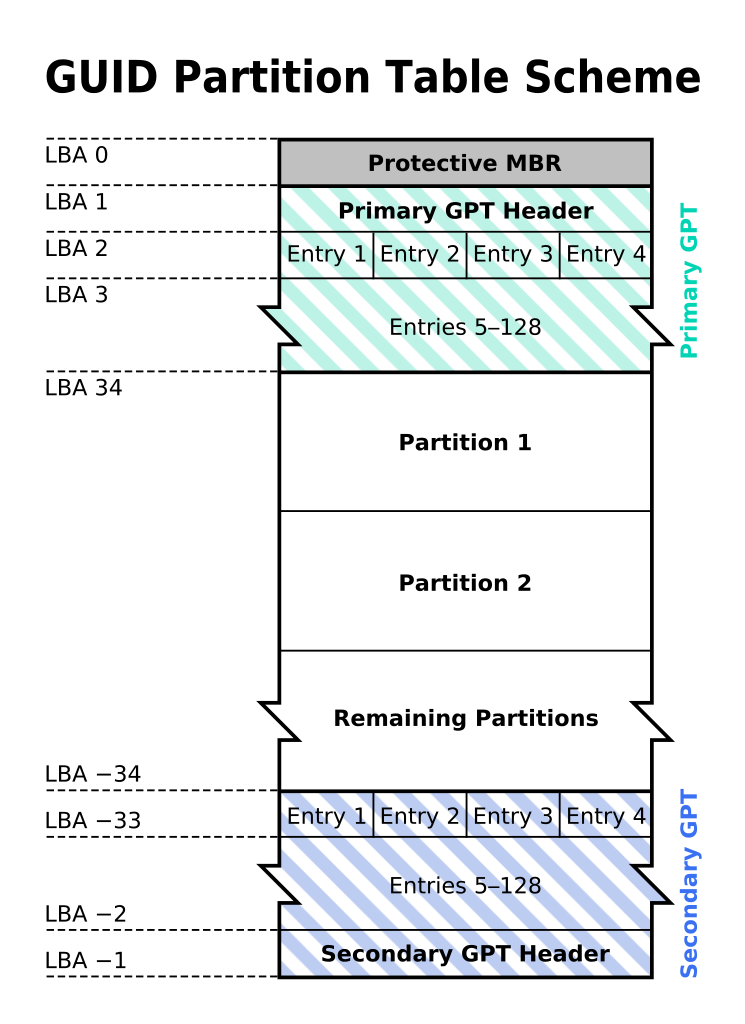
\includegraphics[scale=0.23,angle=270]{images/gpt.png}
        \captionsetup{labelformat=empty,labelsep=none}
        \transparent{0.4}%
    \end{figure}
\end{frame}


\begin{frame}[fragile]
  \frametitle{5.8 Exercise: Investigate disk with  strange PT}
    \begin{itemize}
        \item Fix the first partition table entry! \texttt{mmls mbr\_ex.raw}
    \end{itemize}
  \begin{lstlisting}[basicstyle=\tiny]
        Slot      Start        End          Length       Description
000:  Meta      0000000000   0000000000   0000000001   Primary Table (#0)
001:  -------   0000000000   0000002049   0000002050   Unallocated
002:  000:000   0000002050   0000067585   0000065536   Win95 FAT32 (0x0c)
003:  000:001   0000067586   0000133119   0000065534   Win95 FAT32 (0x0c)
004:  000:002   0000133120   0000262142   0000129023   Win95 FAT32 (0x0c)
005:  -------   0000262143   0000262143   0000000001   Unallocated
  \end{lstlisting}
    \begin{itemize}
        \item Search for partition 1 signature
    \end{itemize}
  \begin{lstlisting}[basicstyle=\tiny]
sigfind -o 510 -l AA55 mbr_ex.raw
  \end{lstlisting}
\end{frame}


\begin{frame}[fragile]
  \frametitle{5.8 Exercise: Investigate disk with  strange PT}
    \begin{itemize}
        \item The fixed partition table:
    \end{itemize}
  \begin{lstlisting}[basicstyle=\tiny]
      Slot      Start        End          Length       Description
000:  Meta      0000000000   0000000000   0000000001   Primary Table (#0)
001:  -------   0000000000   0000002047   0000002048   Unallocated
002:  000:000   0000002048   0000067583   0000065536   Win95 FAT32 (0x0c)
003:  -------   0000067584   0000067585   0000000002   Unallocated
004:  000:001   0000067586   0000133119   0000065534   Win95 FAT32 (0x0c)
005:  000:002   0000133120   0000262142   0000129023   Win95 FAT32 (0x0c)
006:  -------   0000262143   0000262143   0000000001   Unallocated
  \end{lstlisting}
    \begin{itemize}
        \item Investigate partition 3 boundaries
    \end{itemize}
  \begin{lstlisting}[basicstyle=\tiny]
dd if=mbr_ex.raw count=2049 | xxd | less
dd if=mbr_ex.raw skip=67583 count=4 | xxd | less
dd if=mbr_ex.raw skip=262142 | xxd | less
  \end{lstlisting}
\end{frame}


\begin{frame}[fragile]
  \frametitle{5.9 VBR - Volume Boot Record - Boot Sector}
  \begin{lstlisting}[basicstyle=\tiny]
# dd if=/dev/sdc1 bs=512 count=1 skip=0 |xxd

0000000: eb58 906d 6b64 6f73 6673 0000 0208 2000  .X.mkdosfs.... .     # 0xeb 0x58 0x90
0000010: 0200 0000 00f8 0000 3e00 f800 0000 0000  ........>.......     # JMP  2+88 NOP
0000030: 0100 0600 0000 0000 0000 0000 0000 0000  ................
0000040: 0000 29a2 20e9 9c46 4154 2020 2020 2020  ..). ..FAT      
0000050: 2020 4641 5433 3220 2020 0e1f be77 7cac    FAT32   ...w|.
0000060: 22c0 740b 56b4 0ebb 0700 cd10 5eeb f032  ".t.V.......^..2
...
...
00001f0: 0000 0000 0000 0000 0000 0000 0000 55aa  ..............U.


0 - 2           Size:  3    Jump to bootstrap code
3 - 10          Size:  8    OEM-ID: mkdosfs
11 - 12         Size:  2    Bytes per sector: 0x0002 -> 0x0200 (little endian)-> 512
13 (0xD)        Size:  1    Sectors per cluster: 0x08 -> 4096 bytes per cluster
50 (0x32) - 51  Size:  2    Boot sector backup: 0x0600 -> 0x0006 -> at sector 6
67 (0x43) - 70  Size:  4    Volume serial number: 0xa220e99c -> 0x9ce920a2
71 (0x47)       Size: 11    Volume label: FAT
82 (0x52)       Size:  8    Partition type: FAT32
90 (0x5A)- 509 (0x1FD)	    Bootstrap code
510 (0x1FE)     Size:  2    Signature: 0x55AA
  \end{lstlisting}
    \begin{itemize}
        \item Demo: Sleuthkit tools: \texttt{mmstat, mmls, fsstat}
    \end{itemize}
\end{frame}








